\subsection{Suivi de murs}
  \subsubsection{Introduction}
  On s'intéresse ici à la programmation d'un robot\footnote{Un robot en Lego
  Mindstorms NXT, accompagné seulement de deux capteurs à ultrasons et
  deux boutons poussoirs.} afin qu'il puisse longer un mur.

  Afin de longer un mur, on peut par exemple poser un capteur à ultrasons sur
  le côté gauche de notre robot. Lorsqu'il détecte qu'il est trop
  éloigné du mur, il tourne légèrement à gauche. Donc s'il ne détecte plus
  de mur à gauche (le mur tourne) le robot va naturellement tourner à gauche.

  Cette méthode donnant des résultats peu probants si la direction initiale du
  robot n'est pas exactement parallèle au mur, on peut ajouter un autre capteur
  à ultrasons à l'avant du robot. Ainsi, on peut tourner désormais à gauche,
  tout en avançant légèrement, dès qu'on détecte que le mur est trop loin; et
  si on se retrouve face à notre mur, alors on tourne vers la droite jusqu'à ne
  plus l'être.

  Ainsi, on peut suivre un mur droit de manière assez régulière.

\subsection{Labyrinthe}\label{sec:laby}
  \subsubsection{Suivi de mur}
    Pour sortir d'un labyrinthe, le suivi de mur est déjà un algorithme
    admissible, il trouvera une solution s'il en existe une. En effet, si on
    n'arrive pas à sortir du labyrinthe en suivant cette méthode, c'est qu'on 
    longe un ilot dans le labyrinthe, ce qui est impossible si l'on vient
    de l'extérieur.

    L'algorithme de Dijkstra et l'algorithme A* (qui est considéré comme une
    extension du premier) sont utilisés pour trouver le chemin le plus court
    permettant de sortir du labyrinthe.

  \subsubsection{Algorithme de Dijkstra}
    L'algorithme de Dijkstra est un algorithme permettant de trouver le plus
    court chemin entre deux sommets d'un graphe (orienté ou non): il est donc
    utile dans le cas du labyrinthe, car celui-ci peut être représenté comme un
    graphe. En effet il suffit de représenter chaque intersection du labyrinthe
    comme un sommet du graphe, et chaque chemin du labyrinthe par une arête du
    graphe comme sur l'illustration suivante:

    \begin{center}
      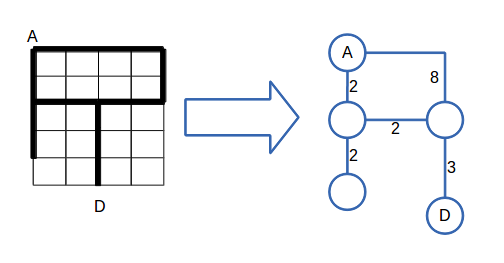
\includegraphics[width=0.55\textwidth]{../slides/jeux/GRO_graph1.png}
    \end{center}

    La complexité de cet algorithme est polynomiale suivant le nombre de sommets
    du graphe.

    Son principe est simple: il parcourt le graphe en gardant en mémoire la
    longueur du chemin le plus court vers chaque sommet.

  \subsubsection{Algorithme A*}
    L'algorithme A* est une amélioration de Dijkstra, qui utilise une heuristique
    pour orienter la recherche.
    Si l'heuristique est bien choisie, il est même possible de s'assurer qu'A*
    donnera bien le résultat optimal (et plus rapidement que Dijkstra).

    Cet algorithme utilise deux listes de nœuds: une liste, dite ouverte, qui
    contient les nœuds explorables et une liste, dite fermée, qui contient les
    nœuds déjà explorés.

    \begin{itemize}
      \item On crée un nœud en lui attribuant un cout heuristique qui
        correspond à la somme du cout du nœud et d'une estimation de la distance de ce
        nœud à l'arrivée.

        Remarque: l'utilisation de ce cout heuristique constitue une différence
        notable avec l'algorithme de Dijkstra, elle permet de s'assurer que
        l'on va toujours plus ou moins dans la bonne direction.

        Par exemple dans un graphe en étoile avec des branches de même taille
        et plusieurs nœuds par branches où l'on part du centre pour rejoindre
        l'extrémité d'une branche l'algorithme de Djkstra explore toutes les
        branches simultanément alors qu'avec l'utilisation du cout heuristique
        on explore directement et uniquement la bonne branche.
      \item On ajoute ce nœud à la liste ouverte.
      \item On prend le nœud qui a le meilleur cout heuristique dans la liste
        ouverte et on l'ajoute à la liste fermée.
      \item On crée les nœuds adjacents et pour chacun d'eux:
        \begin{itemize}
          \item leur cout est égal à la somme des couts de leurs prédécesseurs
            et du cout entre les deux;
          \item si l'un d'eux est présent dans la liste ouverte on vérifie si
            ce nouveau chemin trouvé est plus rapide. Si c'est le cas on
            remplace celui qui est dans la liste ouverte par le nouveau sinon
            on oublie le nouveau;
          \item s'il est déjà dans la liste fermée c'est qu'il a déjà été
            traité ou qu'il est en train d'être traité donc on l'oublie;
          \item et s'il n'est ni dans la liste ouverte ni dans la liste fermée,
            on l'ajoute à la liste ouverte.
        \end{itemize}
    \end{itemize}
	
    À la fin, en remontant tous les prédécesseurs, on remonte le chemin le plus
    court.

  \subsection{Construction du labyrinthe par le robot}
    Cependant pour pouvoir appliquer ces algorithmes il faut connaitre le
    labyrinthe, afin de construire son graphe.

    Or ceci est loin d'être évident: le robot n'ayant aucun moyen de se repérer
    avec précision dans l'espace, il lui faudrait se baser sur la vitesse des
    moteurs pour déterminer sa position. Mais cette méthode peut se révéler
    très mauvaise notamment si le robot change souvent la vitesse d'un moteur
    (pour tourner par exemple) ou s'arrête souvent: il va alors accumuler les
    erreurs de position. De plus, le sol et les roues n'étant pas parfaits, le 
    robot dérape relativement souvent, ce qui augmente encore les erreurs.

  \subsection{Conclusion}
    Le problème du robot dans un labyrinthe est assez simple en théorie. Mais,
    comme souvent, la pratique est bien plus compliquée, car en plus des
    mathématiques qui sont derrière ce problème, viennent des problèmes
    intrinsèques aux robots.

% vim: shiftwidth=2 softtabstop=2 tabstop=2 spell spelllang=fr
